\documentclass{article}
\usepackage[T1]{fontenc} % codificação da fonte em 8-bits
\usepackage[utf8]{inputenc} % acentuação direta
\usepackage[brazil]{babel} % em portugues brasileiro
\usepackage[normalem]{ulem}
\useunder{\uline}{\ul}{}
\usepackage{graphicx}
\usepackage[utf8]{inputenc}
\usepackage{fullpage}
\usepackage{listings}
\usepackage{xcolor}
\usepackage{amsmath}
\usepackage{amssymb}
\usepackage{url}
\usepackage{hyperref}
\usepackage[linesnumbered,ruled,vlined]{algorithm2e}
% \usepackage{enumitem}
\usepackage[shortlabels]{enumitem}
\usepackage{listings}
\lstset { %
    language=C++,
    backgroundcolor=\color{black!5}, % set backgroundcolor
    basicstyle=\footnotesize,% basic font setting
}


\definecolor{mygreen}{rgb}{0,0.6,0}

% set the default code style
\lstset{
    language=C++,
    frame=tb, % draw a frame at the top and bottom of the code block
    tabsize=4, % tab space width
    showstringspaces=false, % don't mark spaces in strings
    numbers=none, % display line numbers on the left
    commentstyle=\color{mygreen}, % comment color
    keywordstyle=\color{blue}, % keyword color
    stringstyle=\color{red}, % string color
    backgroundcolor=\color{black!5}, % set backgroundcolor
    basicstyle=\footnotesize,% basic font setting
    literate = {-}{-}1, % <------ trick for '-' in shell commands
}

\parindent0in
\pagestyle{plain}
\thispagestyle{plain}

\newcommand{\assignment}{Lista 2}
\newcommand{\duedate}{Março 20, 2022}


\title{Lista 2}
\date{}

\begin{document}

Fundação Getulio Vargas\hfill\\
Estruturas de Dados\hfill\textbf{\assignment}\\
Prof.\ Jorge Poco\hfill\textbf{Entrega:} \duedate\\
\smallskip\hrule\bigskip

{\let\newpage\relax\maketitle}
\maketitle

\section*{Parte 1 - Questões Teóricas}

\paragraph{Problema 1.}(12 pontos)
\begin{enumerate}[label*=1.\arabic*.]
  \item (6 pontos) Considere a árvore enraizada da \autoref{fig:fig1}(a). Desenhe uma figura mostrando sua representação na forma “primeiro filho/próximo irmão”.
  \item (6 pontos) Considere a árvore enraizada da \autoref{fig:fig1}(b) representada na forma “primeiro filho/próximo irmão”. Desenhe uma figura mostrando a árvore enraizada equivalente.
\end{enumerate}

\begin{figure}[!h]
  \centering
    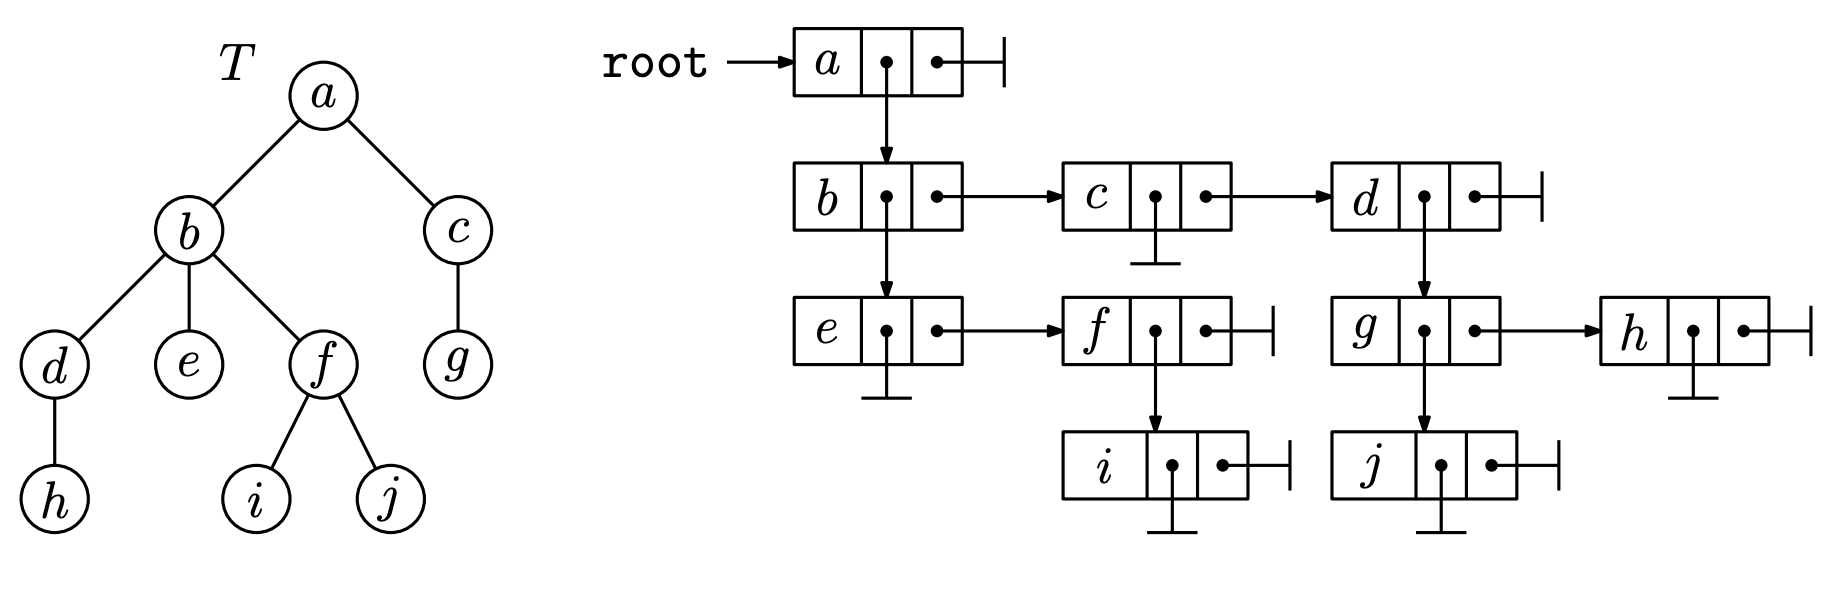
\includegraphics[width=.6\textwidth]{figures/fig1.png}
    \caption{Árvore enraízada a partir de árvore "primeiro-filho/próximo irmão" e vice-versa.}
  \label{fig:fig1}
\end{figure}


\textbf{Resposta 1:}

\paragraph{Problema 2.} (8 pontos) Desenhe a árvore binária da \autoref{fig:fig2}(a) com os fios da ordem (\emph{inorder-threads}) adicionados.

\begin{figure}[!h]
  \centering
    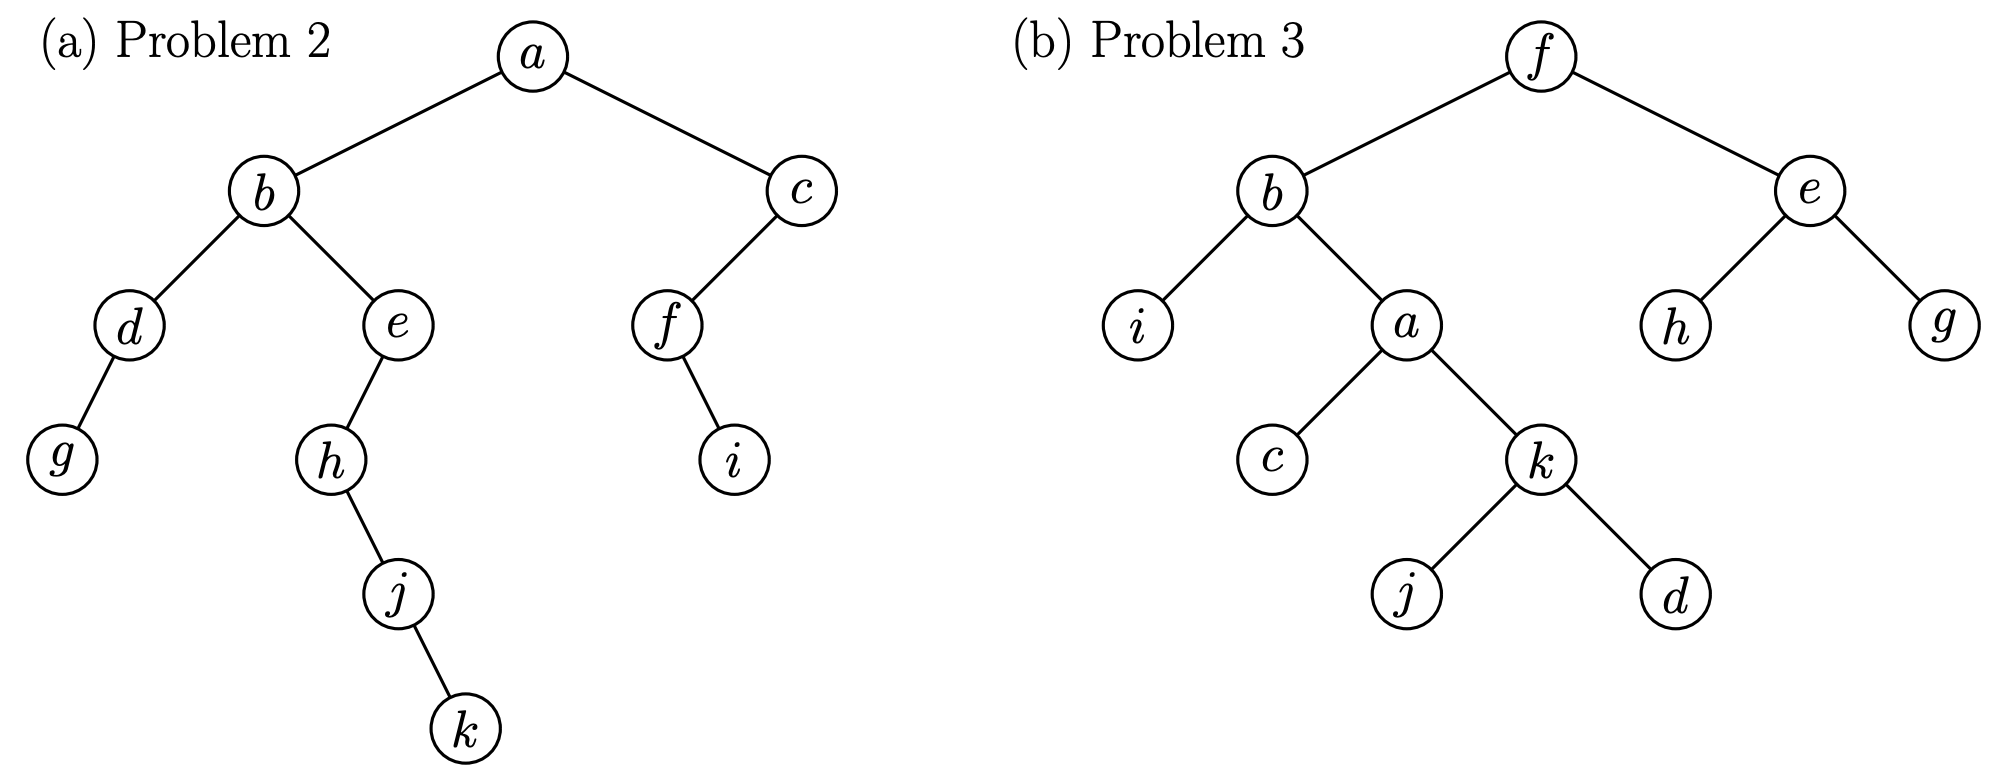
\includegraphics[width=.6\textwidth]{figures/fig2.png}
    \caption{Adicionando \textit{inorder threads} para uma árvore binária e uma árvore binária completa.}
  \label{fig:fig2}
\end{figure}



\textbf{Resposta 2:}
 
\paragraph{Problema 3} (15 pontos) Você tem uma árvore binária completa, onde cada nó é rotulado com um letra. (Lembre-se de que uma árvore binária está cheia se cada nó não folha tiver exatamente dois filhos.) Ao longo deste problema, restringimos a atenção às árvores binárias completas.

% \begin{enumerate}[(a)]
\begin{enumerate}[label*=3.\arabic*.]
    \item (3 pontos) Alguém executou uma travessia \textit{postorder} e forneceu uma lista com os nomes dos nós. (Por exemplo, na árvore mostrada na \autoref{fig:fig2}(b), isso é $(i, c, j, d, k, a, b, h, g, e, f)$. É possível recuperar a estrutura da árvore binária completa exclusivamente da sequência \textit{postorder}? Se sim, explique como apresentando um algoritmo para fazê-lo. Se não, desenhe duas árvores binárias completas rotuladas onde as listas de \textit{postorder} são as mesmas.
    \item (3 pontos) Repita (3.1), mas dessa vez a lista foi modificada para que cada o nó folha foi “marcado” para distinguir as folhas dos nós internos. (Por exemplo, na árvore mostrada na Fig.~\ref{fig:fig2}(b), se usarmos "$\star$" para indicar uma folha, isso seria $(i*, c*, j*, d*, k, a, b, h*, g*, e, f)$.
    \item (3 pontos) Repita (3.1), mas desta vez para um temos a lista do percurso \textit{inorder} de uma árvore binária completa. (Para exemplo, na árvore mostrada na \autoref{fig:fig2}(b), isso seria $(i, b, c, a, j, k, d, f, h, e, g)$.
    \item (4 pontos) Repita (3.2), mas desta vez para um temos a lista do percurso \textit{inorder} de uma árvore binária completa. (Para exemplo, na árvore mostrada na \autoref{fig:fig2}(b), isso seria $(i*, b, c*, a, j*, k, d*, f, h*, e, g*)$. 
    \item (4 pontos) Não pediremos que você resolva o caso restante (com uma sequência de um percurso \textit{preorder}), mas suponha que você discuta o caso (3.1) com seu melhor amigo (sequência \textit{preorder} sem os nós interno marcados). (Vocês dois suspeitam que o malvado professor pode colocar essa questão em um exame futuro.) Este amigo anuncia que a resposta é “não” e informa que existe um contra-exemplo simples de 6 nós. Sem sequer ver o contra-exemplo, você diz ao seu amigo que isso está errado! Como é isso possível? (Assuma para este problema que você não é um médium.)
\end{enumerate}

\textbf{Resposta 3:}

\paragraph{Problema 4} (15 pontos) São dadas duas matrizes $n \times n$ $A$ e $B$, onde (seguindo a  convenção de C++) as linhas e colunas são indexadas de $0$ a $n-1$. Seu produto $A \cdot B$ é uma  matriz $n \times n$ $C$, onde para $0 \leq i$, $j \leq n-1$, $C[i,j]=\sum_{k=0}^{n-1}A[i,k]\cdot B[k,j]$.

\begin{figure}[!h]
  \centering  
    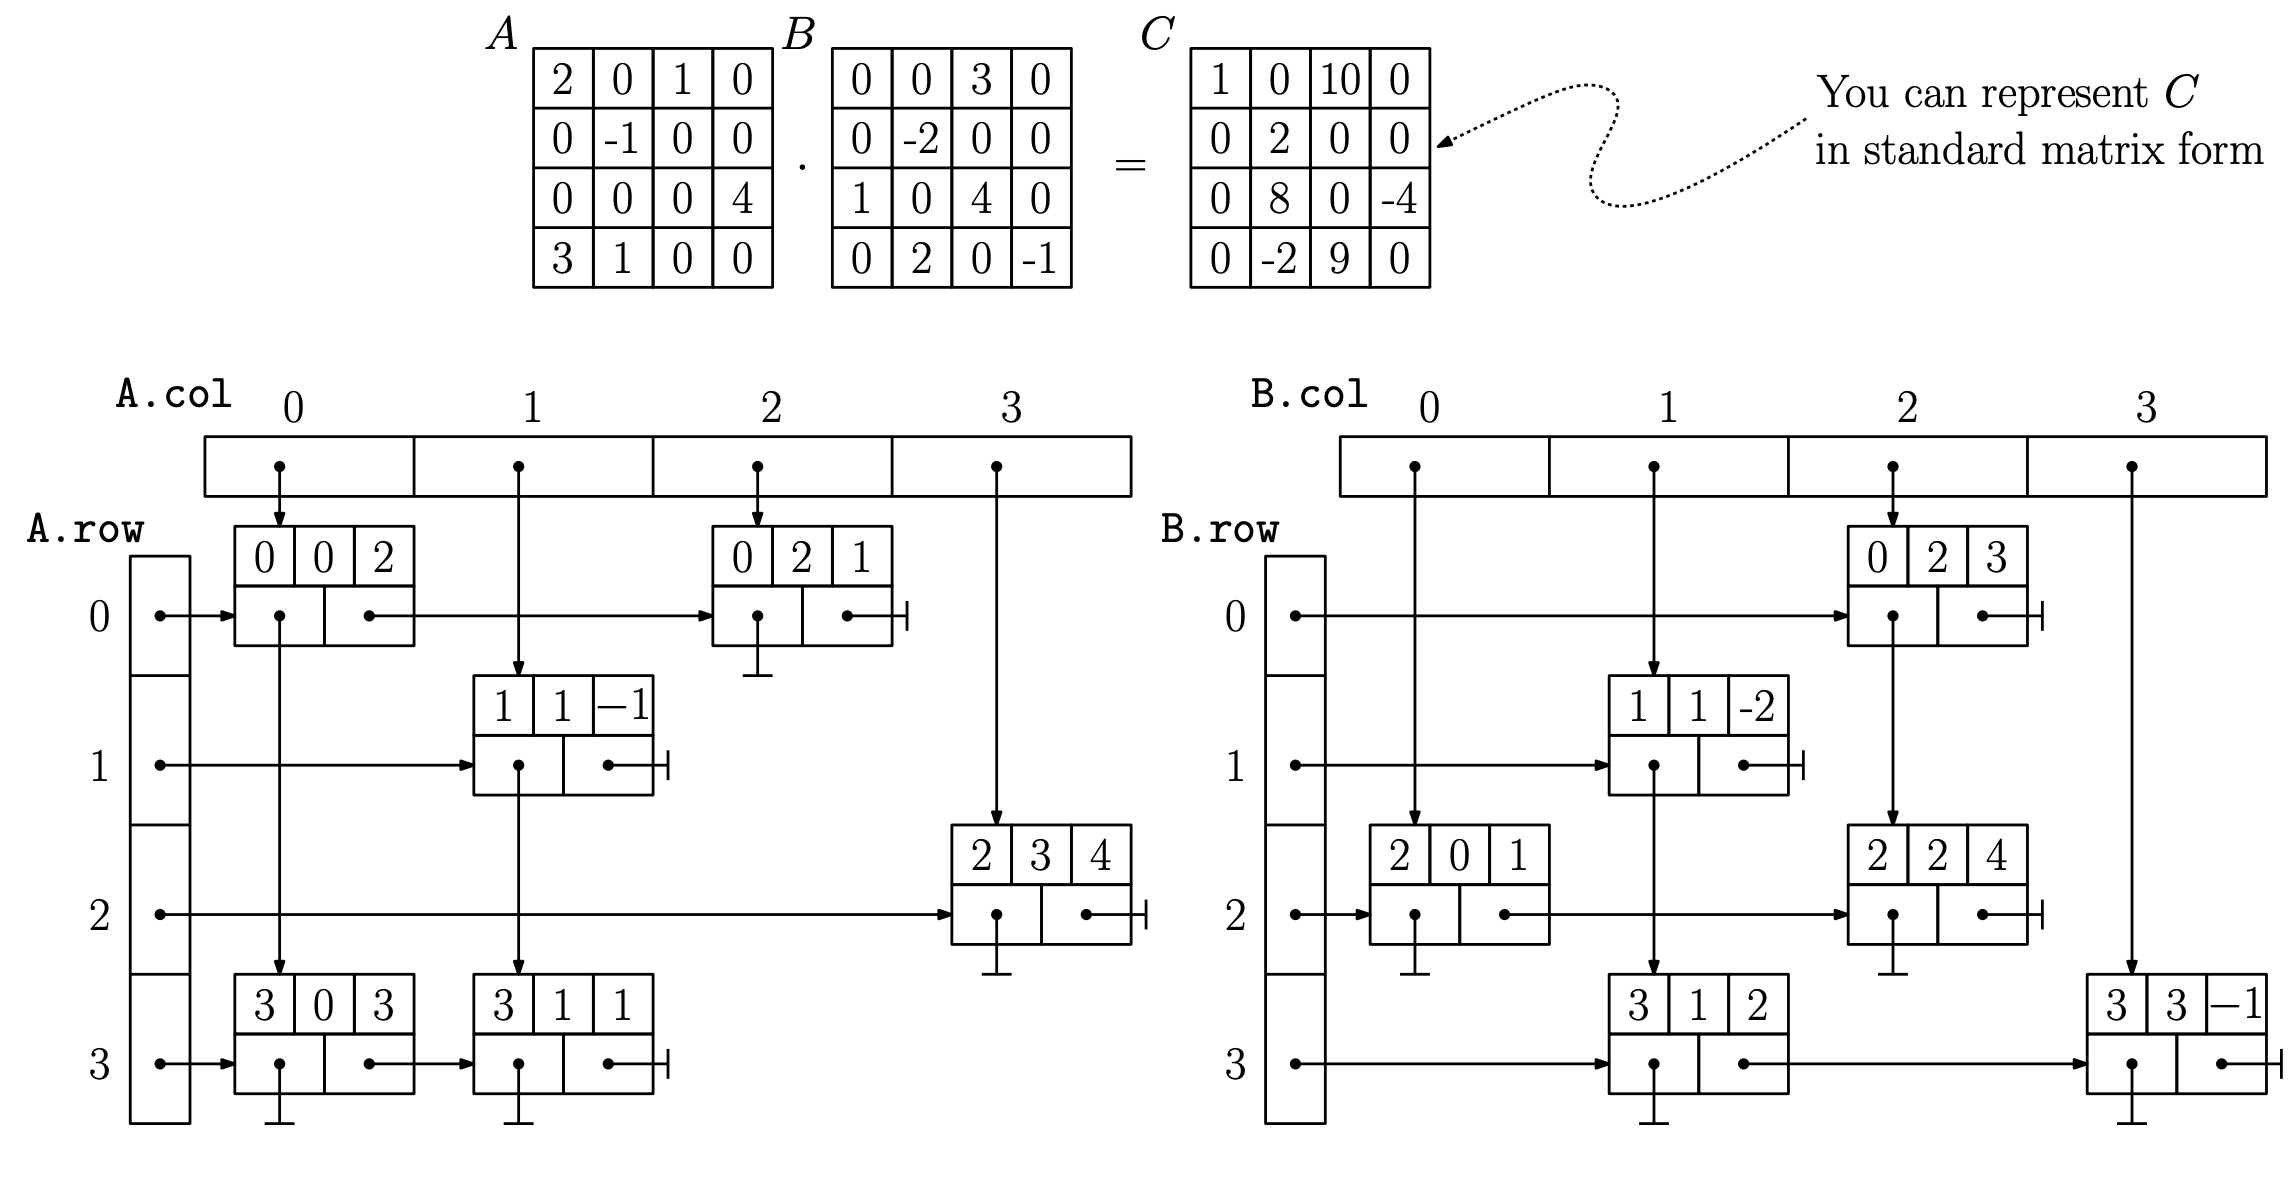
\includegraphics[width=.9\textwidth]{figures/matrix.png}
  \caption{Multiplicação de matriz esparsa.}
  \label{fig:matrix}
\end{figure}


\begin{enumerate}[label*=4.\arabic*.]
  \item (5 pontos) Assuma que $A$ e $B$ são representadas por matrizes esparsas (ver Lecture 4 e \autoref{fig:matrix}). Apresente um algoritmo eficiente para o cálculo do produto $A\cdot B$. \\
  Para simplificar, você pode assumir que a matriz de saída $C$ é representada como uma matriz bidimensional $n \times n$ , que foi inicializada com zeros.
  Para tornar possível a generalize sua solução para o caso esparso, você deve preencher as entradas não zero de $C$ em ordem seqüencial (por exemplo, de cima para baixo e da esquerda para a direita).
  \item (3 pontos) Dê o tempo de execução de seu algoritmo em termos das seguintes quantidades: $n$, $N_A$ e $N_B$, onde $N_A$ e $N_B$ são os números de entradas não zeradas nas matrizes $A$ e $B$, respectivamente. (Ou seja, declare qual é o tempo de execução assimptótico e apresente uma prova ou explicação convincente de sua limitação. \textbf{Dica}: No caso especial quando as matrizes são densas, ou seja, $N_A = N_B = n^2$, o tempo de execução deve ser $O(n^3)$).
\end{enumerate}

\textbf{Resposta 4:}

\newpage
\section*{Parte 2 - Tarefa de programação}

\paragraph{Quake Heaps:}

Este é a primeira tarefa (dividida em mais partes) para implementar uma estrutura de dados interessante chamada de \textit{Quake Heap}. Tal como acontece com \textit{heaps} padrão, esta estrutura de dados implementa uma prioridade fila. Tal estrutura de dados armazena pares chave-valor, onde as chaves são de um tipo ordenável (como \texttt{ints}, \texttt{floats} ou \texttt{strings}). 
No mínimo, uma fila de prioridade suporta o operações de \textit{insert} (adicionar um novo par chave-valor) e \textit{extrair-min} (remover a entrada com o menor chave e retornar seu valor associado).

\begin{figure}[!h]
    \centering
    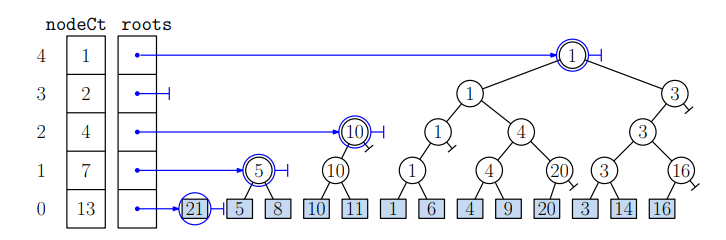
\includegraphics[width = 0.8\linewidth]{figures/fig5.png}
    \caption{Uma \textit{Quake Heap} armazenando as chaves $(21, 5, 8, 10, 11, 1, 6, 4, 9, 20, 3, 14, 16)$.}
    \label{fig:fig5}
\end{figure}

O exemplo mais famoso de heap é a b\textit{inary heap}, que é a estrutura de dados usada por \textit{HeapSort}. Existem inúmeras variantes, que fornecem desempenho aprimorado para vários operações, notadamente a de diminuir uma chave. A \textit{Quake Heap} é uma dessas variantes. Foi desenvolvido por Timothy Chan (descrito neste \href{http://tmc.web.engr.illinois.edu/heap_ianfest.pdf}{artigo}) como uma alternativa mais simples para a \textit{Fibonacci Heap}. Suporta inserção e chaves decrescentes em tempo $O(1)$, e suporta \textit{extract-min} em $O(log n)$ tempo amortizado. 
Na primeira parte da tarefa, implementaremos apenas uma parte das funcionalidades do \textit{Quake Heap}.

A classe \texttt{QuakeHeap} funcionará com tipos genéricos, um tipo de chave
e um tipo de valor. O tipo de chave deve ser ordenável, e assumimos que ambos podem ser convertidos para strings com \texttt{to\_string}. 
O \texttt{QuakeHeap}  é representado como uma coleção de árvores binárias, onde cada nó armazena um par de valores-chave. Os nós dessas árvores são organizados em níveis. Todas as folhas residem no nível 0, e cada chave na \textit{heap} é armazenada em exatamente uma folha de alguma árvore. (Por exemplo, na \autoref{fig:fig5},
as chaves consistem nas 13 chaves nos nós de folha azul.)

Cada nó interno tem um filho esquerdo e um filho direito opcional. O valor da sua chave é igual ao do seu filho da esquerda. Se o filho direito existir, seu valor de chave será maior ou igual ao filho esquerdo. Cada raíz contém o menor valor de chave sobre todas as folhas, que (pela nossa regra que a chave esquerda é menor) é o da folha mais à esquerda. Segue que a menor chave no \textit{heap} será armazenada em uma das raízes (mas geralmente não sabemos qual).

Cada nó armazena um par chave-valor, ponteiros filho esquerdo e direito, ponteiro pai e seu nível. 

Mantemos dois \texttt{arrays} adicionais organizados por nível:
\begin{itemize}
    \item \texttt{roots[lev]}: Uma lista encadeada contendo referências às raízes da árvore do nível \texttt{lev}. (Nós recomendo implementar isso como um lista encadeada de nós (\texttt{std::list})).
    \item \texttt{node\_counter[lev]}: Armazena o número total de nós no nível \texttt{lev}.
\end{itemize}

\texttt{Nodes} e \texttt{Locators}: Os principais objetos que estão sendo manipulados são os nós da \texttt{QuakeHeap}. Como mencionado acima, cada nó armazena um par chave-valor, links filho esquerdo e direito, link pai,
e seu nível na árvore. Os nós no nível 0 são folhas, portanto, ambos os links filho são nulos. Um nó raiz (em qualquer nível) tem um link pai de nulo. C++ fornece uma maneira elegante de definir uma classe aninhada a outra, assim faremos o \texttt{Node}, dentro da classe \texttt{QuakeHeap}.

Um detalhe complicado em qualquer estrutura de \textit{heap} que suporte diminuir o valor de uma chave é que precisamos de um mecanismo para identificar a entrada cuja chave desejamos diminuir. Quando inserimos um valor-chave
par, criamos um novo nó folha. Como o \texttt{Node} é um objeto protegido dentro do \texttt{QuakeHeap}, não podemos retornar um ponteiro diretamente para ele. Em vez disso, criamos um objeto público especial, chamado \texttt{Locator},
para incluir uma referência a este nó folha recém-inserido. A função \texttt{insert} retorna um localizador referenciando o nó recém-criado. 

Operações: Para esta parte do projeto, começaremos implementando as funções básicas necessárias inserir chaves. Aqui está uma lista das operações que você deve implementar.

\begin{itemize}
    \item  \texttt{QuakeHeap(int n\_levels)} (10 pontos) : Constrói uma \texttt{QuakeHeap} vazia. O parâmetro \texttt{n\_Level} indica o número de níveis a serem alocados em seus \texttt{arrays roots} e \texttt{node\_counter}. Você deve inicializar essas estruturas e outros atributos que sua classe use.
    \item \texttt{void Clear()}  (10 pontos): Isso redefine a estrutura para seu estado inicial. Em particular, ele redefine a contagem \texttt{node\_counter} para zero e limpa \texttt{roots}.
    \item \texttt{Locator Insert(T1 key, T2 value)}  (20 pontos):  Isso insere o par chave-valor (\textit{key, value}) na \textit{heap}. Isso cria uma árvore “trivial” que consiste em um único nó raiz no nível 0, que armazena esse par chave-valor. Ele insere este nó no array \texttt{roots[0]}. Ele retorna um \texttt{Locator} (veja acima) referenciando o nó folha recém-criado.
    \item \texttt{vector<string> ListHeap()}  (10 pontos): Esta operação lista o conteúdo de sua estrutura em um \texttt{vector<string>}. O formato preciso é importante, pois verificamos a correção comparando com os nossos resultados. Enumere os níveis da árvore de baixo para cima. Para cada nível, faça o seguinte:
    \begin{itemize}
        \item Se a contagem de nós para este nível for zero, pule este nível e vá para o próximo. Caso contrário, ordene os nós raíz deste nível por seu valor de chave.
        \item Gere um cabeçalho de nível na forma de uma string"\texttt{{lev: xxx nodeCt: yyy}}” e adicione no \texttt{vector}. Aqui, “xxx” é o índice de nível e “yyy” é a contagem de nós para este nível. Por exemplo, se houver quatro nós no nível dois, isso gera a string, “\texttt{{lev: 2 nodeCt: 4}}”.
        \item  Para cada nó raiz \texttt{r} na lista de raízes para este nível, enumere os nós deste árvore com base em uma travessia de \textit{preorder}. Para cada nó \texttt{u} visitado nesta travessia, fazemos:
        \begin{itemize}
            \item Se \texttt{u.level >= 1} gere a string \texttt{"(" + u.key + ")"}. Visite recursivamente \texttt{u.left} e \texttt{u.right}. 
            \item Se \texttt{u.level = 0} gere a string \texttt{"[" + u.key + " " + u.value + "]"} e retorne.
            \item Se \texttt{u = nullptr}, retorne a string \texttt{"[null]"}.
        \end{itemize}
    \end{itemize}
\end{itemize}

Código base: Como na tarefa anterior, forneceremos o código esqueleto na classe no \textit{Github Classroom}. Iremos fornecer os arquivos \textit{headers} e o nosso \textit{tester} e os arquivos de texto de teste. Você só precisa implementar a \texttt{QuakeHeap} com as funções listadas acima. 

Nós vamos avaliar seu trabalho utilizando o seguinte comando para compilar:
\begin{lstlisting}[language=bash]
g++ -std=c++11 tester.cc -o tester
\end{lstlisting}

Caso o código não compile, a nota será 0.
Após a compilação, nós iremos realizar testes baseados em arquivos de texto (que estão dentro da pasta \texttt{src/tests}), utilizaremos o comando:

\begin{lstlisting}[language=bash]
tester <tests/test01-input.txt >tests/test01-output.txt
\end{lstlisting}
    
Com isso, será gerado um arquivo dentro da pastas tests de output, você deve comparar o \texttt{tests/test01-output.txt} com o arquivo \texttt{tests/test01-expected.txt} com o comando:

\begin{lstlisting}[language=bash]
diff tests/test01-output.txt tests/test01-expected.txt
\end{lstlisting}

Nós iremos considerar como um erro caso o comando \texttt{diff} aponte diferenças entre os arquivos (incluindo espaços em branco). 
O número 01 pode ser trocado por 02 e 03 para testar com os outros arquivos de teste. 

Uma outra avaliação será o estilo do código. Você deve formatar seu código baseado no estilo recomendo pelo  Google, de acordo com a referência no seguinte \href{https://google.github.io/styleguide/cppguide.html}{link}. 
%
Utilizaremos \textit{cpplint} para verificar o seu código. A cada \textit{alerta} referente a formatação, será retirado 5 pontos da nota. Você também pode verificar com as instruções no \href{https://github.com/cpplint/cpplint}{link}. Para executar, em um terminal use o comando:  

\begin{lstlisting}[language=bash]
cpplint --extensions=cc,hpp,h --header=h --repository=. tester.cc quake_heap.h quake_heap.hpp
\end{lstlisting}


\newpage
\appendix

\section{Detalhes avaliação}
Uma pergunta comum é "quanto detalhe é esperado nas respostas?", algumas orientações são:
%
\paragraph{Provar vs. Mostrar:}
Se lhe pedirmos para “provar” algo, estamos à procura de uma prova bem estruturada. Se você estiver aplicando a indução, tenha cuidado para distinguir seu(s) caso(s) básico(s) e indicar qual é a sua hipótese de indução. Se lhe pedirmos para “mostrar”, “explicar” ou “justificar”, estaremos geralmente apenas esperando uma explicação em português. Se você não tiver certeza, por favor, verifique.

\paragraph{Algoritmo vs. Pseudocódigo:} Quando pedimos um “algoritmo” estamos esperando uma descrição em alto nível de algum processo computacional, geralmente em uma combinação de português e notação matemática (por exemplo, “classifique as $n$ chaves e localize $x$ usando busca binária”). Para pseudocódigo, nós estão esperando uma descrição passo a passo mais detalhada que se pareça muito mais com C++ (por exemplo, “\texttt{Node q = p.left}”). Lembre-se de que você está escrevendo seu código para ser lido por um humano, e não por um compilador. Por favor, omita detalhes irrelevantes que são sintaxes de C++. Mesmo que não solicitemos explicitamente, sempre que você fornecer um algoritmo ou pseudocódigo, você deve sempre fornecer uma breve explicação em português. Isso ajuda o avaliador a entender quais são suas intenções, e se houver um pequeno erro em seu código, muitas vezes podemos usar seu explicação para entender quais eram suas reais intenções.

\section{Adição de Matriz Esparsa}

Os estudantes muitas vezes me perguntam quantos detalhes eu espero para perguntas que envolvam dar um algoritmo. Sempre que lhe for pedido que apresente um "algoritmo", você deve apresentar o seguinte (mesmo que eu não peça tudo isso explicitamente):

\begin{itemize}[noitemsep]
  \item Uma breve explicação em português
  \item Apresentar o próprio algoritmo, tipicamente em pseudo-código
  \item Se não for óbvio, justifique brevemente a correção do algoritmo
  \item Faça uma breve análise do tempo de funcionamento
\end{itemize}

A seguir, apresento uma solução de amostra para o problema da adição de matriz com a matriz esparsa representação. Vamos supor que nos são dadas duas matrizes esparsas $A$ e $B$ (ver Lecture 4), e nosso objetivo é calcular sua soma matricial $C$. Para simplificar, vamos supor que $C$ é dada como uma matriz $n \times n$ padrão, que é inicializada a zero, e tudo o que precisamos fazer é preencher são as entradas não zeradas. Seguindo as convenções de C++, assumimos que as linhas e colunas são indexados de $0$ a $n-1$. Lembramos que na representação de matriz esparsa, nos são dados dois $n$-element arrays, chame-lhes \texttt{row[]} e \texttt{col[]}, onde \texttt{row[i]} é o chefe (\emph{head}) de uma lista encadeada das entradas na linha \texttt{i}, e \texttt{col[j]} é o cabeçalho (\emph{head}) de uma lista encadeada de nós na coluna \texttt{j}. Estas listas encadeadas são ordenadas por ordem crescente de índices. Cada entrada de matriz diferente de zero é representada por um nó contendo as seguintes informações:

\begin{lstlisting}
Class Node {
  int row;        // indice da linha
  int col;        // indice da coluna
  float value;    // o valor desta entrada da matriz
  Node *rowNext;  // a proxima entrada (da esquerda para a direita) nesta linha
  Node *colNext;  // a proxima entrada (de cima para baixo) nesta coluna
}
\end{lstlisting}


O algoritmo itera através de cada linha $0 \leq i \leq n - 1$, e depois itera de forma coordenada através das duas listas ligadas \texttt{A.row[i]} e \texttt{B.row[i]}. Se ambas as entradas estiverem na mesma coluna, calculamos sua soma e a armazenamos em \texttt{C}. Caso contrário, copiamos o valor que se encontra no índice menor da coluna. Após processarmos uma entrada, avançamos para o próximo elemento da lista encadeada. Quando chegamos ao final de qualquer uma das listas, simplesmente copiamos as demais entradas da outra lista para as entradas apropriadas em \texttt{C}.

Aqui está o pseudo-código. Omitiremos tanto quanto possível as especificações do tipo.

\begin{lstlisting}
void sparseAddition(SparseMatrix A, SparseMatrix B, float C[][])
  for (i = 0 to n-1) {                   // iterate through all the rows
    ap = A.row[i]                       // head of A's ith row
    bp = B.row[i]                       // head of B's ith row
    while (ap != NULL && bp != NULL) {   // while entries remain in both rows
      if (ap.col < bp.col) {           // A's entry comes next?
        C[i][ap.col] = ap.value        //copy to C and advance
        ap = ap.rowNext
      } else if (bp.col < ap.col) {     // B's entry comes next?
        C[i][bp.col] = bp.value // copy to C and advance
        bp = bp.rowNext
      } else { // (ap.col == bp.col)   // both in the same column?
        C[i][ap.col] = ap.value + bp.value // put sum in C and advance
        ap = ap.rowNext
        bp = bp.rowNext
      }
    }
    // At this point, only one list has elements remaining
    while (ap != null) {                 // copy any remainder from A to C
      C[i][ap.col] = ap.value
      ap = ap.rowNext
    }
    while (bp != null) {                 // copy any remainder from B to C
      C[i][bp.col] = bp.value
      bp = bp.rowNext
    }
  }
\end{lstlisting}

A correção decorre do fato de que os dois indicadores \texttt{ap} e \texttt{bp} se movem em coordenação, de modo que um nunca fica muito à frente do outro. Para obter o tempo de execução, observe que visitamos cada um dos nós das representações de matriz esparsa para \texttt{A} e \texttt{B} exatamente uma vez (quando estamos processando sua fila). Como há $N_A$ nós em A e $N_B$ em $B$, isto leva tempo $O(N_A + N_B)$. Entretanto, mesmo que estas quantidades sejam ambas zero, ainda assim será necessário acessar cada uma das $n$ entradas de \texttt{A.row} e \texttt{B.row}. Assim, o tempo total de execução é $O(n+ N_A + N_B)$.




\end{document}






